\documentclass[tikz,border=1.5mm]{standalone}
\usepackage[T1]{fontenc}
\usepackage[utf8]{inputenc}
\usepackage{lmodern}
\usepackage[scaled=1]{helvet}
\renewcommand{\familydefault}{\sfdefault}
\usepackage{amssymb,textcomp}
\usepackage{sansmath}
\usetikzlibrary{arrows.meta,calc}
\renewcommand{\arraystretch}{1.12}
\setlength{\tabcolsep}{2.6pt}
\tikzset{
  F3/.style={font=\fontsize{4.2}{5}\selectfont},
  F4/.style={font=\fontsize{5}{6}\selectfont},
  F4b/.style={font=\fontsize{5}{6}\selectfont\bfseries},
  F5/.style={font=\fontsize{5.6}{6.6}\selectfont},
  F5b/.style={font=\fontsize{5.8}{6.8}\selectfont\bfseries},
  F6/.style={font=\fontsize{6.4}{7.4}\selectfont},
  F6b/.style={font=\fontsize{6.8}{8}\selectfont\bfseries},
  enc/.style={densely dashed,line width=0.4pt},
}
\begin{document}
\sansmath
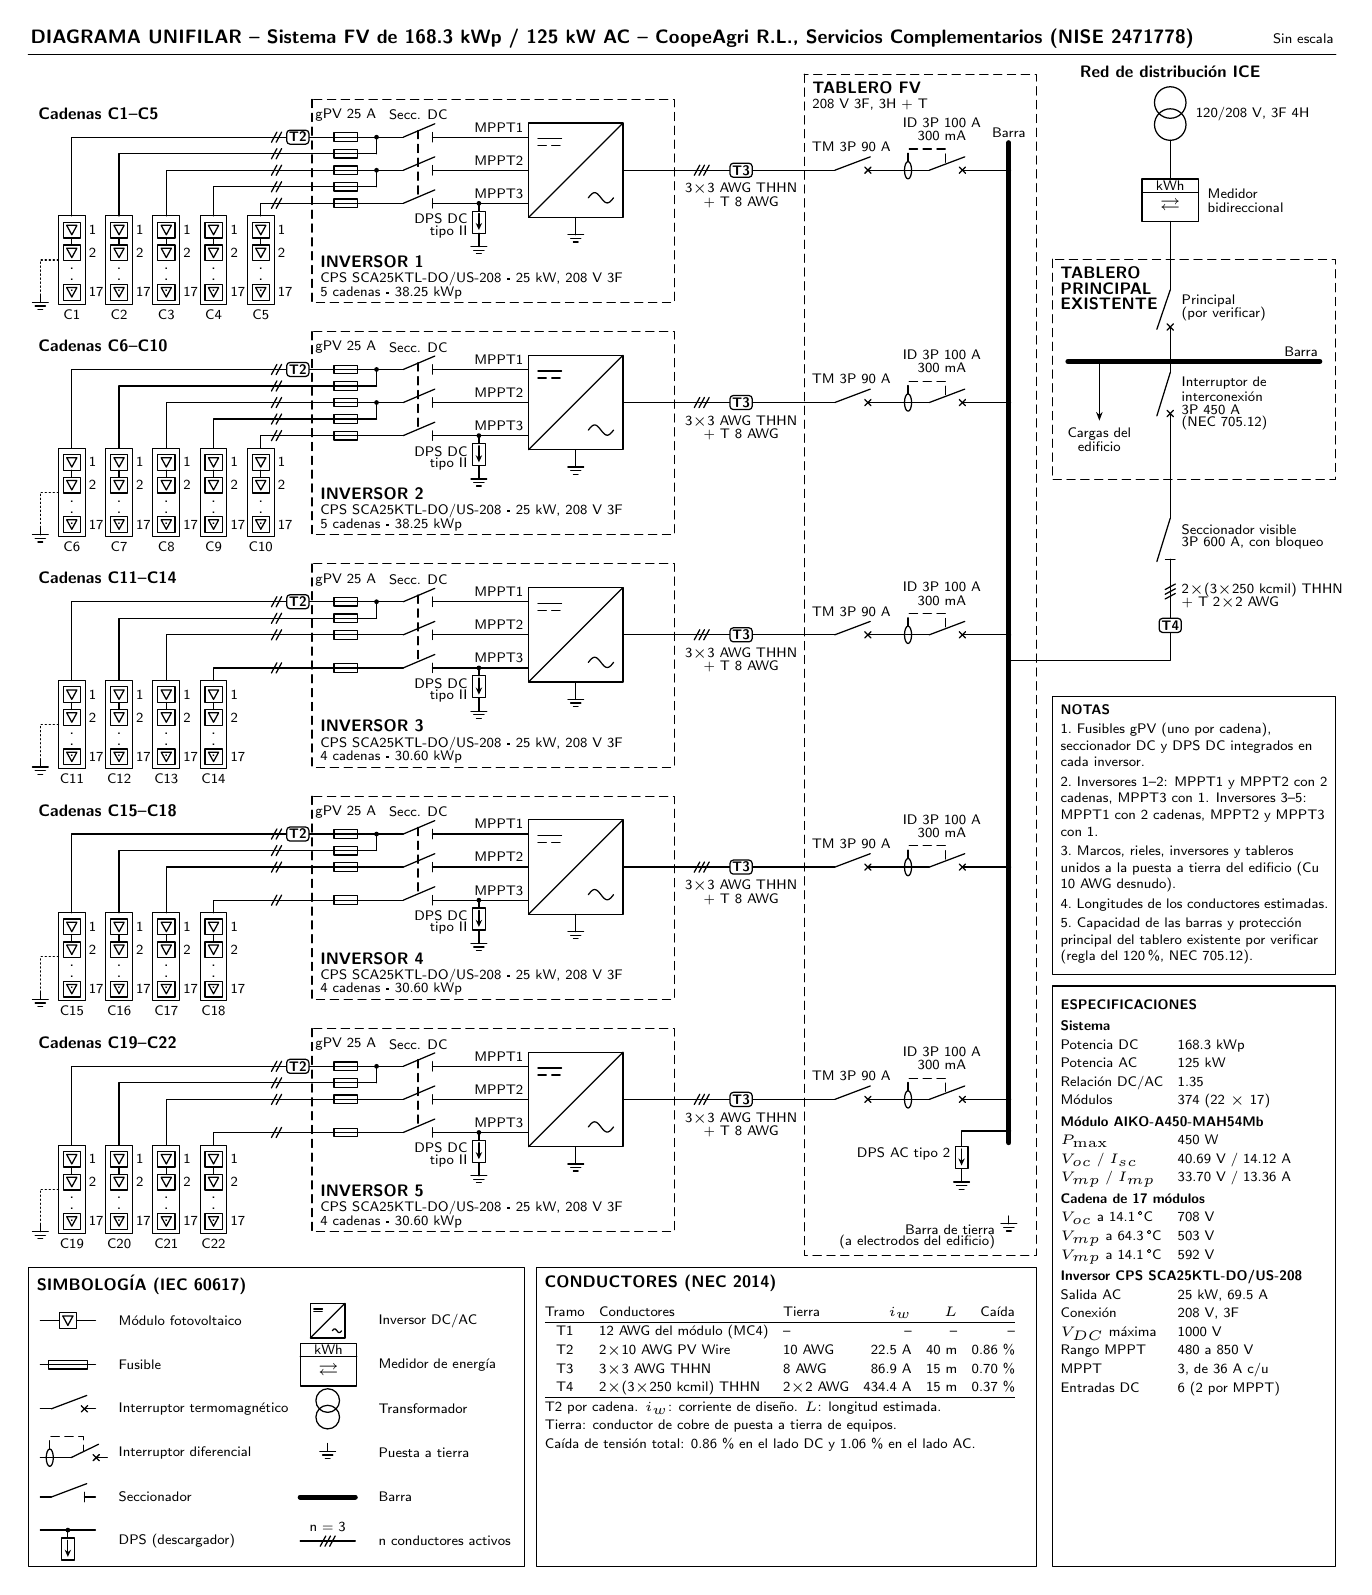
\begin{tikzpicture}[line width=0.45pt,line cap=round,line join=round]
\node[F6b,anchor=west,inner sep=0.5pt,] at (0.000,0.000) {DIAGRAMA UNIFILAR \textendash{} Sistema FV de 168.3 kWp / 125 kW AC \textendash{} CoopeAgri R.L., Servicios Complementarios (NISE 2471778)};
\node[F4,anchor=east,inner sep=0.5pt,] at (16.600,0.000) {Sin escala};
\draw[line width=0.6pt] (0.000,-0.200) -- (16.600,-0.200);
\node[F5b,anchor=west,inner sep=0.5pt,] at (0.100,-0.950) {Cadenas C1\textendash C5};
\draw[line width=0.35pt] (0.380,-2.250) rectangle (0.720,-3.370);
\draw[fill=white] (0.440,-2.530) rectangle (0.660,-2.330);
\draw (0.485,-2.370) -- (0.615,-2.370) -- (0.550,-2.490) -- cycle;
\node[F3,anchor=west,inner sep=0.5pt,] at (0.740,-2.430) {1};
\draw[fill=white] (0.440,-2.820) rectangle (0.660,-2.620);
\draw (0.485,-2.660) -- (0.615,-2.660) -- (0.550,-2.780) -- cycle;
\node[F3,anchor=west,inner sep=0.5pt,] at (0.740,-2.720) {2};
\draw[fill=white] (0.440,-3.320) rectangle (0.660,-3.120);
\draw (0.485,-3.160) -- (0.615,-3.160) -- (0.550,-3.280) -- cycle;
\node[F3,anchor=west,inner sep=0.5pt,] at (0.740,-3.220) {17};
\draw[] (0.550,-2.530) -- (0.550,-2.620);
\node[F5,anchor=center,inner sep=0.5pt,] at (0.550,-2.960) {$\vdots$};
\node[F4,anchor=center,inner sep=0.5pt,] at (0.550,-3.500) {C1};
\draw[] (0.550,-2.250) -- (0.550,-1.250) -- (3.780,-1.250);
\draw[] (3.085,-1.315) -- (3.155,-1.185);
\draw[] (3.145,-1.315) -- (3.215,-1.185);
\draw[line width=0.35pt] (0.980,-2.250) rectangle (1.320,-3.370);
\draw[fill=white] (1.040,-2.530) rectangle (1.260,-2.330);
\draw (1.085,-2.370) -- (1.215,-2.370) -- (1.150,-2.490) -- cycle;
\node[F3,anchor=west,inner sep=0.5pt,] at (1.340,-2.430) {1};
\draw[fill=white] (1.040,-2.820) rectangle (1.260,-2.620);
\draw (1.085,-2.660) -- (1.215,-2.660) -- (1.150,-2.780) -- cycle;
\node[F3,anchor=west,inner sep=0.5pt,] at (1.340,-2.720) {2};
\draw[fill=white] (1.040,-3.320) rectangle (1.260,-3.120);
\draw (1.085,-3.160) -- (1.215,-3.160) -- (1.150,-3.280) -- cycle;
\node[F3,anchor=west,inner sep=0.5pt,] at (1.340,-3.220) {17};
\draw[] (1.150,-2.530) -- (1.150,-2.620);
\node[F5,anchor=center,inner sep=0.5pt,] at (1.150,-2.960) {$\vdots$};
\node[F4,anchor=center,inner sep=0.5pt,] at (1.150,-3.500) {C2};
\draw[] (1.150,-2.250) -- (1.150,-1.460) -- (3.780,-1.460);
\draw[] (3.085,-1.525) -- (3.155,-1.395);
\draw[] (3.145,-1.525) -- (3.215,-1.395);
\draw[line width=0.35pt] (1.580,-2.250) rectangle (1.920,-3.370);
\draw[fill=white] (1.640,-2.530) rectangle (1.860,-2.330);
\draw (1.685,-2.370) -- (1.815,-2.370) -- (1.750,-2.490) -- cycle;
\node[F3,anchor=west,inner sep=0.5pt,] at (1.940,-2.430) {1};
\draw[fill=white] (1.640,-2.820) rectangle (1.860,-2.620);
\draw (1.685,-2.660) -- (1.815,-2.660) -- (1.750,-2.780) -- cycle;
\node[F3,anchor=west,inner sep=0.5pt,] at (1.940,-2.720) {2};
\draw[fill=white] (1.640,-3.320) rectangle (1.860,-3.120);
\draw (1.685,-3.160) -- (1.815,-3.160) -- (1.750,-3.280) -- cycle;
\node[F3,anchor=west,inner sep=0.5pt,] at (1.940,-3.220) {17};
\draw[] (1.750,-2.530) -- (1.750,-2.620);
\node[F5,anchor=center,inner sep=0.5pt,] at (1.750,-2.960) {$\vdots$};
\node[F4,anchor=center,inner sep=0.5pt,] at (1.750,-3.500) {C3};
\draw[] (1.750,-2.250) -- (1.750,-1.670) -- (3.780,-1.670);
\draw[] (3.085,-1.735) -- (3.155,-1.605);
\draw[] (3.145,-1.735) -- (3.215,-1.605);
\draw[line width=0.35pt] (2.180,-2.250) rectangle (2.520,-3.370);
\draw[fill=white] (2.240,-2.530) rectangle (2.460,-2.330);
\draw (2.285,-2.370) -- (2.415,-2.370) -- (2.350,-2.490) -- cycle;
\node[F3,anchor=west,inner sep=0.5pt,] at (2.540,-2.430) {1};
\draw[fill=white] (2.240,-2.820) rectangle (2.460,-2.620);
\draw (2.285,-2.660) -- (2.415,-2.660) -- (2.350,-2.780) -- cycle;
\node[F3,anchor=west,inner sep=0.5pt,] at (2.540,-2.720) {2};
\draw[fill=white] (2.240,-3.320) rectangle (2.460,-3.120);
\draw (2.285,-3.160) -- (2.415,-3.160) -- (2.350,-3.280) -- cycle;
\node[F3,anchor=west,inner sep=0.5pt,] at (2.540,-3.220) {17};
\draw[] (2.350,-2.530) -- (2.350,-2.620);
\node[F5,anchor=center,inner sep=0.5pt,] at (2.350,-2.960) {$\vdots$};
\node[F4,anchor=center,inner sep=0.5pt,] at (2.350,-3.500) {C4};
\draw[] (2.350,-2.250) -- (2.350,-1.880) -- (3.780,-1.880);
\draw[] (3.085,-1.945) -- (3.155,-1.815);
\draw[] (3.145,-1.945) -- (3.215,-1.815);
\draw[line width=0.35pt] (2.780,-2.250) rectangle (3.120,-3.370);
\draw[fill=white] (2.840,-2.530) rectangle (3.060,-2.330);
\draw (2.885,-2.370) -- (3.015,-2.370) -- (2.950,-2.490) -- cycle;
\node[F3,anchor=west,inner sep=0.5pt,] at (3.140,-2.430) {1};
\draw[fill=white] (2.840,-2.820) rectangle (3.060,-2.620);
\draw (2.885,-2.660) -- (3.015,-2.660) -- (2.950,-2.780) -- cycle;
\node[F3,anchor=west,inner sep=0.5pt,] at (3.140,-2.720) {2};
\draw[fill=white] (2.840,-3.320) rectangle (3.060,-3.120);
\draw (2.885,-3.160) -- (3.015,-3.160) -- (2.950,-3.280) -- cycle;
\node[F3,anchor=west,inner sep=0.5pt,] at (3.140,-3.220) {17};
\draw[] (2.950,-2.530) -- (2.950,-2.620);
\node[F5,anchor=center,inner sep=0.5pt,] at (2.950,-2.960) {$\vdots$};
\node[F4,anchor=center,inner sep=0.5pt,] at (2.950,-3.500) {C5};
\draw[] (2.950,-2.250) -- (2.950,-2.090) -- (3.780,-2.090);
\draw[] (3.085,-2.155) -- (3.155,-2.025);
\draw[] (3.145,-2.155) -- (3.215,-2.025);
\draw[densely dotted] (0.380,-2.810) -- (0.150,-2.810) -- (0.150,-3.250);
\draw[] (0.150,-3.250) -- (0.150,-3.350);
\draw[] (0.050,-3.350) -- (0.250,-3.350);
\draw[] (0.085,-3.395) -- (0.215,-3.395);
\draw[] (0.120,-3.440) -- (0.180,-3.440);
\node[F4b,draw,rounded corners=1.2pt,fill=white,inner sep=0.8pt] at (3.420,-1.250) {T2};
\draw[enc] (3.600,-0.770) rectangle (8.200,-3.350);
\node[F4,anchor=center,inner sep=0.5pt,] at (4.030,-0.970) {gPV 25 A};
\node[F4,anchor=center,inner sep=0.5pt,] at (4.950,-0.970) {Secc. DC};
\draw[] (3.780,-1.250) -- (4.280,-1.250);
\draw[fill=white] (3.880,-1.305) rectangle (4.180,-1.195);
\draw[] (3.880,-1.250) -- (4.180,-1.250);
\draw[] (4.280,-1.250) -- (4.420,-1.250);
\draw[] (3.780,-1.460) -- (4.280,-1.460);
\draw[fill=white] (3.880,-1.515) rectangle (4.180,-1.405);
\draw[] (3.880,-1.460) -- (4.180,-1.460);
\draw[] (4.280,-1.460) -- (4.420,-1.460);
\draw[] (3.780,-1.670) -- (4.280,-1.670);
\draw[fill=white] (3.880,-1.725) rectangle (4.180,-1.615);
\draw[] (3.880,-1.670) -- (4.180,-1.670);
\draw[] (4.280,-1.670) -- (4.420,-1.670);
\draw[] (3.780,-1.880) -- (4.280,-1.880);
\draw[fill=white] (3.880,-1.935) rectangle (4.180,-1.825);
\draw[] (3.880,-1.880) -- (4.180,-1.880);
\draw[] (4.280,-1.880) -- (4.420,-1.880);
\draw[] (3.780,-2.090) -- (4.280,-2.090);
\draw[fill=white] (3.880,-2.145) rectangle (4.180,-2.035);
\draw[] (3.880,-2.090) -- (4.180,-2.090);
\draw[] (4.280,-2.090) -- (4.420,-2.090);
\draw[] (4.420,-1.250) -- (4.420,-1.460);
\fill (4.420,-1.250) circle (0.03);
\draw[] (4.420,-1.250) -- (4.620,-1.250);
\draw[] (4.620,-1.250) -- (4.760,-1.250);
\draw[] (4.760,-1.250) -- (5.160,-1.080);
\draw[] (5.130,-1.250) -- (5.270,-1.250);
\draw[] (5.130,-1.310) -- (5.130,-1.190);
\draw[] (5.270,-1.250) -- (6.350,-1.250);
\node[F3,anchor=south east,inner sep=0.5pt,] at (6.310,-1.210) {MPPT1};
\draw[] (4.420,-1.670) -- (4.420,-1.880);
\fill (4.420,-1.670) circle (0.03);
\draw[] (4.420,-1.670) -- (4.620,-1.670);
\draw[] (4.620,-1.670) -- (4.760,-1.670);
\draw[] (4.760,-1.670) -- (5.160,-1.500);
\draw[] (5.130,-1.670) -- (5.270,-1.670);
\draw[] (5.130,-1.730) -- (5.130,-1.610);
\draw[] (5.270,-1.670) -- (6.350,-1.670);
\node[F3,anchor=south east,inner sep=0.5pt,] at (6.310,-1.630) {MPPT2};
\draw[] (4.420,-2.090) -- (4.620,-2.090);
\draw[] (4.620,-2.090) -- (4.760,-2.090);
\draw[] (4.760,-2.090) -- (5.160,-1.920);
\draw[] (5.130,-2.090) -- (5.270,-2.090);
\draw[] (5.130,-2.150) -- (5.130,-2.030);
\draw[] (5.270,-2.090) -- (6.350,-2.090);
\node[F3,anchor=south east,inner sep=0.5pt,] at (6.310,-2.050) {MPPT3};
\draw[densely dashed] (4.945,-1.165) -- (4.945,-2.005);
\fill (5.720,-2.090) circle (0.03);
\draw[] (5.720,-2.090) -- (5.720,-2.190);
\draw (5.640,-2.190) rectangle (5.800,-2.470);
\draw[-{Stealth[length=0.9mm,width=0.8mm]}] (5.720,-2.220) -- (5.720,-2.430);
\draw[] (5.720,-2.470) -- (5.720,-2.540);
\draw[] (5.720,-2.540) -- (5.720,-2.640);
\draw[] (5.620,-2.640) -- (5.820,-2.640);
\draw[] (5.655,-2.685) -- (5.785,-2.685);
\draw[] (5.690,-2.730) -- (5.750,-2.730);
\node[F4,anchor=east,inner sep=0.5pt,] at (5.600,-2.290) {DPS DC};
\node[F4,anchor=east,inner sep=0.5pt,] at (5.600,-2.450) {tipo II};
\draw[fill=white] (6.350,-2.270) rectangle (7.550,-1.070);
\draw[] (6.350,-2.270) -- (7.550,-1.070);
\draw[] (6.470,-1.270) -- (6.770,-1.270);
\draw[densely dashed] (6.470,-1.360) -- (6.770,-1.360);
\draw plot[domain=0:1,samples=25,smooth] ({7.109999999999999+0.32*\x},{-2.02+0.065*sin(360*\x)});
\draw[] (6.950,-2.270) -- (6.950,-2.390);
\draw[] (6.950,-2.390) -- (6.950,-2.490);
\draw[] (6.850,-2.490) -- (7.050,-2.490);
\draw[] (6.885,-2.535) -- (7.015,-2.535);
\draw[] (6.920,-2.580) -- (6.980,-2.580);
\node[F5b,anchor=north west,inner sep=0.5pt,] at (3.680,-2.730) {INVERSOR 1};
\node[F4,anchor=north west,inner sep=0.5pt,] at (3.680,-2.940) {CPS SCA25KTL-DO/US-208 \textperiodcentered{} 25 kW, 208 V 3F};
\node[F4,anchor=north west,inner sep=0.5pt,] at (3.680,-3.120) {5 cadenas \textperiodcentered{} 38.25 kWp};
\draw[] (7.550,-1.670) -- (10.100,-1.670);
\draw[] (8.455,-1.735) -- (8.525,-1.605);
\draw[] (8.515,-1.735) -- (8.585,-1.605);
\draw[] (8.575,-1.735) -- (8.645,-1.605);
\node[F4b,draw,rounded corners=1.2pt,fill=white,inner sep=0.8pt] at (9.050,-1.670) {T3};
\node[F4,anchor=north,inner sep=0.5pt,] at (9.050,-1.810) {3$\times$3 AWG THHN};
\node[F4,anchor=north,inner sep=0.5pt,] at (9.050,-1.980) {+ T 8 AWG};
\draw[] (10.100,-1.670) -- (10.240,-1.670);
\draw[] (10.240,-1.670) -- (10.690,-1.500);
\draw[] (10.660,-1.670) -- (10.800,-1.670);
\draw[] (10.620,-1.710) -- (10.700,-1.630);
\draw[] (10.620,-1.630) -- (10.700,-1.710);
\node[F4,anchor=south,inner sep=0.5pt,] at (10.450,-1.460) {TM 3P 90 A};
\draw[] (10.800,-1.670) -- (11.050,-1.670);
\draw[] (11.050,-1.670) -- (11.300,-1.670);
\draw (11.170,-1.670) ellipse (0.045 and 0.11);
\draw[] (11.300,-1.670) -- (11.440,-1.670);
\draw[] (11.440,-1.670) -- (11.890,-1.500);
\draw[] (11.860,-1.670) -- (12.000,-1.670);
\draw[] (11.820,-1.710) -- (11.900,-1.630);
\draw[] (11.820,-1.630) -- (11.900,-1.710);
\draw[densely dashed] (11.170,-1.560) -- (11.170,-1.400) -- (11.650,-1.400) -- (11.650,-1.585);
\node[F4,anchor=south,inner sep=0.5pt,] at (11.600,-1.320) {300 mA};
\node[F4,anchor=south,inner sep=0.5pt,] at (11.600,-1.150) {ID 3P 100 A};
\draw[] (12.000,-1.670) -- (12.450,-1.670);
\fill (12.450,-1.670) circle (0.03);
\node[F5b,anchor=west,inner sep=0.5pt,] at (0.100,-3.900) {Cadenas C6\textendash C10};
\draw[line width=0.35pt] (0.380,-5.200) rectangle (0.720,-6.320);
\draw[fill=white] (0.440,-5.480) rectangle (0.660,-5.280);
\draw (0.485,-5.320) -- (0.615,-5.320) -- (0.550,-5.440) -- cycle;
\node[F3,anchor=west,inner sep=0.5pt,] at (0.740,-5.380) {1};
\draw[fill=white] (0.440,-5.770) rectangle (0.660,-5.570);
\draw (0.485,-5.610) -- (0.615,-5.610) -- (0.550,-5.730) -- cycle;
\node[F3,anchor=west,inner sep=0.5pt,] at (0.740,-5.670) {2};
\draw[fill=white] (0.440,-6.270) rectangle (0.660,-6.070);
\draw (0.485,-6.110) -- (0.615,-6.110) -- (0.550,-6.230) -- cycle;
\node[F3,anchor=west,inner sep=0.5pt,] at (0.740,-6.170) {17};
\draw[] (0.550,-5.480) -- (0.550,-5.570);
\node[F5,anchor=center,inner sep=0.5pt,] at (0.550,-5.910) {$\vdots$};
\node[F4,anchor=center,inner sep=0.5pt,] at (0.550,-6.450) {C6};
\draw[] (0.550,-5.200) -- (0.550,-4.200) -- (3.780,-4.200);
\draw[] (3.085,-4.265) -- (3.155,-4.135);
\draw[] (3.145,-4.265) -- (3.215,-4.135);
\draw[line width=0.35pt] (0.980,-5.200) rectangle (1.320,-6.320);
\draw[fill=white] (1.040,-5.480) rectangle (1.260,-5.280);
\draw (1.085,-5.320) -- (1.215,-5.320) -- (1.150,-5.440) -- cycle;
\node[F3,anchor=west,inner sep=0.5pt,] at (1.340,-5.380) {1};
\draw[fill=white] (1.040,-5.770) rectangle (1.260,-5.570);
\draw (1.085,-5.610) -- (1.215,-5.610) -- (1.150,-5.730) -- cycle;
\node[F3,anchor=west,inner sep=0.5pt,] at (1.340,-5.670) {2};
\draw[fill=white] (1.040,-6.270) rectangle (1.260,-6.070);
\draw (1.085,-6.110) -- (1.215,-6.110) -- (1.150,-6.230) -- cycle;
\node[F3,anchor=west,inner sep=0.5pt,] at (1.340,-6.170) {17};
\draw[] (1.150,-5.480) -- (1.150,-5.570);
\node[F5,anchor=center,inner sep=0.5pt,] at (1.150,-5.910) {$\vdots$};
\node[F4,anchor=center,inner sep=0.5pt,] at (1.150,-6.450) {C7};
\draw[] (1.150,-5.200) -- (1.150,-4.410) -- (3.780,-4.410);
\draw[] (3.085,-4.475) -- (3.155,-4.345);
\draw[] (3.145,-4.475) -- (3.215,-4.345);
\draw[line width=0.35pt] (1.580,-5.200) rectangle (1.920,-6.320);
\draw[fill=white] (1.640,-5.480) rectangle (1.860,-5.280);
\draw (1.685,-5.320) -- (1.815,-5.320) -- (1.750,-5.440) -- cycle;
\node[F3,anchor=west,inner sep=0.5pt,] at (1.940,-5.380) {1};
\draw[fill=white] (1.640,-5.770) rectangle (1.860,-5.570);
\draw (1.685,-5.610) -- (1.815,-5.610) -- (1.750,-5.730) -- cycle;
\node[F3,anchor=west,inner sep=0.5pt,] at (1.940,-5.670) {2};
\draw[fill=white] (1.640,-6.270) rectangle (1.860,-6.070);
\draw (1.685,-6.110) -- (1.815,-6.110) -- (1.750,-6.230) -- cycle;
\node[F3,anchor=west,inner sep=0.5pt,] at (1.940,-6.170) {17};
\draw[] (1.750,-5.480) -- (1.750,-5.570);
\node[F5,anchor=center,inner sep=0.5pt,] at (1.750,-5.910) {$\vdots$};
\node[F4,anchor=center,inner sep=0.5pt,] at (1.750,-6.450) {C8};
\draw[] (1.750,-5.200) -- (1.750,-4.620) -- (3.780,-4.620);
\draw[] (3.085,-4.685) -- (3.155,-4.555);
\draw[] (3.145,-4.685) -- (3.215,-4.555);
\draw[line width=0.35pt] (2.180,-5.200) rectangle (2.520,-6.320);
\draw[fill=white] (2.240,-5.480) rectangle (2.460,-5.280);
\draw (2.285,-5.320) -- (2.415,-5.320) -- (2.350,-5.440) -- cycle;
\node[F3,anchor=west,inner sep=0.5pt,] at (2.540,-5.380) {1};
\draw[fill=white] (2.240,-5.770) rectangle (2.460,-5.570);
\draw (2.285,-5.610) -- (2.415,-5.610) -- (2.350,-5.730) -- cycle;
\node[F3,anchor=west,inner sep=0.5pt,] at (2.540,-5.670) {2};
\draw[fill=white] (2.240,-6.270) rectangle (2.460,-6.070);
\draw (2.285,-6.110) -- (2.415,-6.110) -- (2.350,-6.230) -- cycle;
\node[F3,anchor=west,inner sep=0.5pt,] at (2.540,-6.170) {17};
\draw[] (2.350,-5.480) -- (2.350,-5.570);
\node[F5,anchor=center,inner sep=0.5pt,] at (2.350,-5.910) {$\vdots$};
\node[F4,anchor=center,inner sep=0.5pt,] at (2.350,-6.450) {C9};
\draw[] (2.350,-5.200) -- (2.350,-4.830) -- (3.780,-4.830);
\draw[] (3.085,-4.895) -- (3.155,-4.765);
\draw[] (3.145,-4.895) -- (3.215,-4.765);
\draw[line width=0.35pt] (2.780,-5.200) rectangle (3.120,-6.320);
\draw[fill=white] (2.840,-5.480) rectangle (3.060,-5.280);
\draw (2.885,-5.320) -- (3.015,-5.320) -- (2.950,-5.440) -- cycle;
\node[F3,anchor=west,inner sep=0.5pt,] at (3.140,-5.380) {1};
\draw[fill=white] (2.840,-5.770) rectangle (3.060,-5.570);
\draw (2.885,-5.610) -- (3.015,-5.610) -- (2.950,-5.730) -- cycle;
\node[F3,anchor=west,inner sep=0.5pt,] at (3.140,-5.670) {2};
\draw[fill=white] (2.840,-6.270) rectangle (3.060,-6.070);
\draw (2.885,-6.110) -- (3.015,-6.110) -- (2.950,-6.230) -- cycle;
\node[F3,anchor=west,inner sep=0.5pt,] at (3.140,-6.170) {17};
\draw[] (2.950,-5.480) -- (2.950,-5.570);
\node[F5,anchor=center,inner sep=0.5pt,] at (2.950,-5.910) {$\vdots$};
\node[F4,anchor=center,inner sep=0.5pt,] at (2.950,-6.450) {C10};
\draw[] (2.950,-5.200) -- (2.950,-5.040) -- (3.780,-5.040);
\draw[] (3.085,-5.105) -- (3.155,-4.975);
\draw[] (3.145,-5.105) -- (3.215,-4.975);
\draw[densely dotted] (0.380,-5.760) -- (0.150,-5.760) -- (0.150,-6.200);
\draw[] (0.150,-6.200) -- (0.150,-6.300);
\draw[] (0.050,-6.300) -- (0.250,-6.300);
\draw[] (0.085,-6.345) -- (0.215,-6.345);
\draw[] (0.120,-6.390) -- (0.180,-6.390);
\node[F4b,draw,rounded corners=1.2pt,fill=white,inner sep=0.8pt] at (3.420,-4.200) {T2};
\draw[enc] (3.600,-3.720) rectangle (8.200,-6.300);
\node[F4,anchor=center,inner sep=0.5pt,] at (4.030,-3.920) {gPV 25 A};
\node[F4,anchor=center,inner sep=0.5pt,] at (4.950,-3.920) {Secc. DC};
\draw[] (3.780,-4.200) -- (4.280,-4.200);
\draw[fill=white] (3.880,-4.255) rectangle (4.180,-4.145);
\draw[] (3.880,-4.200) -- (4.180,-4.200);
\draw[] (4.280,-4.200) -- (4.420,-4.200);
\draw[] (3.780,-4.410) -- (4.280,-4.410);
\draw[fill=white] (3.880,-4.465) rectangle (4.180,-4.355);
\draw[] (3.880,-4.410) -- (4.180,-4.410);
\draw[] (4.280,-4.410) -- (4.420,-4.410);
\draw[] (3.780,-4.620) -- (4.280,-4.620);
\draw[fill=white] (3.880,-4.675) rectangle (4.180,-4.565);
\draw[] (3.880,-4.620) -- (4.180,-4.620);
\draw[] (4.280,-4.620) -- (4.420,-4.620);
\draw[] (3.780,-4.830) -- (4.280,-4.830);
\draw[fill=white] (3.880,-4.885) rectangle (4.180,-4.775);
\draw[] (3.880,-4.830) -- (4.180,-4.830);
\draw[] (4.280,-4.830) -- (4.420,-4.830);
\draw[] (3.780,-5.040) -- (4.280,-5.040);
\draw[fill=white] (3.880,-5.095) rectangle (4.180,-4.985);
\draw[] (3.880,-5.040) -- (4.180,-5.040);
\draw[] (4.280,-5.040) -- (4.420,-5.040);
\draw[] (4.420,-4.200) -- (4.420,-4.410);
\fill (4.420,-4.200) circle (0.03);
\draw[] (4.420,-4.200) -- (4.620,-4.200);
\draw[] (4.620,-4.200) -- (4.760,-4.200);
\draw[] (4.760,-4.200) -- (5.160,-4.030);
\draw[] (5.130,-4.200) -- (5.270,-4.200);
\draw[] (5.130,-4.260) -- (5.130,-4.140);
\draw[] (5.270,-4.200) -- (6.350,-4.200);
\node[F3,anchor=south east,inner sep=0.5pt,] at (6.310,-4.160) {MPPT1};
\draw[] (4.420,-4.620) -- (4.420,-4.830);
\fill (4.420,-4.620) circle (0.03);
\draw[] (4.420,-4.620) -- (4.620,-4.620);
\draw[] (4.620,-4.620) -- (4.760,-4.620);
\draw[] (4.760,-4.620) -- (5.160,-4.450);
\draw[] (5.130,-4.620) -- (5.270,-4.620);
\draw[] (5.130,-4.680) -- (5.130,-4.560);
\draw[] (5.270,-4.620) -- (6.350,-4.620);
\node[F3,anchor=south east,inner sep=0.5pt,] at (6.310,-4.580) {MPPT2};
\draw[] (4.420,-5.040) -- (4.620,-5.040);
\draw[] (4.620,-5.040) -- (4.760,-5.040);
\draw[] (4.760,-5.040) -- (5.160,-4.870);
\draw[] (5.130,-5.040) -- (5.270,-5.040);
\draw[] (5.130,-5.100) -- (5.130,-4.980);
\draw[] (5.270,-5.040) -- (6.350,-5.040);
\node[F3,anchor=south east,inner sep=0.5pt,] at (6.310,-5.000) {MPPT3};
\draw[densely dashed] (4.945,-4.115) -- (4.945,-4.955);
\fill (5.720,-5.040) circle (0.03);
\draw[] (5.720,-5.040) -- (5.720,-5.140);
\draw (5.640,-5.140) rectangle (5.800,-5.420);
\draw[-{Stealth[length=0.9mm,width=0.8mm]}] (5.720,-5.170) -- (5.720,-5.380);
\draw[] (5.720,-5.420) -- (5.720,-5.490);
\draw[] (5.720,-5.490) -- (5.720,-5.590);
\draw[] (5.620,-5.590) -- (5.820,-5.590);
\draw[] (5.655,-5.635) -- (5.785,-5.635);
\draw[] (5.690,-5.680) -- (5.750,-5.680);
\node[F4,anchor=east,inner sep=0.5pt,] at (5.600,-5.240) {DPS DC};
\node[F4,anchor=east,inner sep=0.5pt,] at (5.600,-5.400) {tipo II};
\draw[fill=white] (6.350,-5.220) rectangle (7.550,-4.020);
\draw[] (6.350,-5.220) -- (7.550,-4.020);
\draw[] (6.470,-4.220) -- (6.770,-4.220);
\draw[densely dashed] (6.470,-4.310) -- (6.770,-4.310);
\draw plot[domain=0:1,samples=25,smooth] ({7.109999999999999+0.32*\x},{-4.97+0.065*sin(360*\x)});
\draw[] (6.950,-5.220) -- (6.950,-5.340);
\draw[] (6.950,-5.340) -- (6.950,-5.440);
\draw[] (6.850,-5.440) -- (7.050,-5.440);
\draw[] (6.885,-5.485) -- (7.015,-5.485);
\draw[] (6.920,-5.530) -- (6.980,-5.530);
\node[F5b,anchor=north west,inner sep=0.5pt,] at (3.680,-5.680) {INVERSOR 2};
\node[F4,anchor=north west,inner sep=0.5pt,] at (3.680,-5.890) {CPS SCA25KTL-DO/US-208 \textperiodcentered{} 25 kW, 208 V 3F};
\node[F4,anchor=north west,inner sep=0.5pt,] at (3.680,-6.070) {5 cadenas \textperiodcentered{} 38.25 kWp};
\draw[] (7.550,-4.620) -- (10.100,-4.620);
\draw[] (8.455,-4.685) -- (8.525,-4.555);
\draw[] (8.515,-4.685) -- (8.585,-4.555);
\draw[] (8.575,-4.685) -- (8.645,-4.555);
\node[F4b,draw,rounded corners=1.2pt,fill=white,inner sep=0.8pt] at (9.050,-4.620) {T3};
\node[F4,anchor=north,inner sep=0.5pt,] at (9.050,-4.760) {3$\times$3 AWG THHN};
\node[F4,anchor=north,inner sep=0.5pt,] at (9.050,-4.930) {+ T 8 AWG};
\draw[] (10.100,-4.620) -- (10.240,-4.620);
\draw[] (10.240,-4.620) -- (10.690,-4.450);
\draw[] (10.660,-4.620) -- (10.800,-4.620);
\draw[] (10.620,-4.660) -- (10.700,-4.580);
\draw[] (10.620,-4.580) -- (10.700,-4.660);
\node[F4,anchor=south,inner sep=0.5pt,] at (10.450,-4.410) {TM 3P 90 A};
\draw[] (10.800,-4.620) -- (11.050,-4.620);
\draw[] (11.050,-4.620) -- (11.300,-4.620);
\draw (11.170,-4.620) ellipse (0.045 and 0.11);
\draw[] (11.300,-4.620) -- (11.440,-4.620);
\draw[] (11.440,-4.620) -- (11.890,-4.450);
\draw[] (11.860,-4.620) -- (12.000,-4.620);
\draw[] (11.820,-4.660) -- (11.900,-4.580);
\draw[] (11.820,-4.580) -- (11.900,-4.660);
\draw[densely dashed] (11.170,-4.510) -- (11.170,-4.350) -- (11.650,-4.350) -- (11.650,-4.535);
\node[F4,anchor=south,inner sep=0.5pt,] at (11.600,-4.270) {300 mA};
\node[F4,anchor=south,inner sep=0.5pt,] at (11.600,-4.100) {ID 3P 100 A};
\draw[] (12.000,-4.620) -- (12.450,-4.620);
\fill (12.450,-4.620) circle (0.03);
\node[F5b,anchor=west,inner sep=0.5pt,] at (0.100,-6.850) {Cadenas C11\textendash C14};
\draw[line width=0.35pt] (0.380,-8.150) rectangle (0.720,-9.270);
\draw[fill=white] (0.440,-8.430) rectangle (0.660,-8.230);
\draw (0.485,-8.270) -- (0.615,-8.270) -- (0.550,-8.390) -- cycle;
\node[F3,anchor=west,inner sep=0.5pt,] at (0.740,-8.330) {1};
\draw[fill=white] (0.440,-8.720) rectangle (0.660,-8.520);
\draw (0.485,-8.560) -- (0.615,-8.560) -- (0.550,-8.680) -- cycle;
\node[F3,anchor=west,inner sep=0.5pt,] at (0.740,-8.620) {2};
\draw[fill=white] (0.440,-9.220) rectangle (0.660,-9.020);
\draw (0.485,-9.060) -- (0.615,-9.060) -- (0.550,-9.180) -- cycle;
\node[F3,anchor=west,inner sep=0.5pt,] at (0.740,-9.120) {17};
\draw[] (0.550,-8.430) -- (0.550,-8.520);
\node[F5,anchor=center,inner sep=0.5pt,] at (0.550,-8.860) {$\vdots$};
\node[F4,anchor=center,inner sep=0.5pt,] at (0.550,-9.400) {C11};
\draw[] (0.550,-8.150) -- (0.550,-7.150) -- (3.780,-7.150);
\draw[] (3.085,-7.215) -- (3.155,-7.085);
\draw[] (3.145,-7.215) -- (3.215,-7.085);
\draw[line width=0.35pt] (0.980,-8.150) rectangle (1.320,-9.270);
\draw[fill=white] (1.040,-8.430) rectangle (1.260,-8.230);
\draw (1.085,-8.270) -- (1.215,-8.270) -- (1.150,-8.390) -- cycle;
\node[F3,anchor=west,inner sep=0.5pt,] at (1.340,-8.330) {1};
\draw[fill=white] (1.040,-8.720) rectangle (1.260,-8.520);
\draw (1.085,-8.560) -- (1.215,-8.560) -- (1.150,-8.680) -- cycle;
\node[F3,anchor=west,inner sep=0.5pt,] at (1.340,-8.620) {2};
\draw[fill=white] (1.040,-9.220) rectangle (1.260,-9.020);
\draw (1.085,-9.060) -- (1.215,-9.060) -- (1.150,-9.180) -- cycle;
\node[F3,anchor=west,inner sep=0.5pt,] at (1.340,-9.120) {17};
\draw[] (1.150,-8.430) -- (1.150,-8.520);
\node[F5,anchor=center,inner sep=0.5pt,] at (1.150,-8.860) {$\vdots$};
\node[F4,anchor=center,inner sep=0.5pt,] at (1.150,-9.400) {C12};
\draw[] (1.150,-8.150) -- (1.150,-7.360) -- (3.780,-7.360);
\draw[] (3.085,-7.425) -- (3.155,-7.295);
\draw[] (3.145,-7.425) -- (3.215,-7.295);
\draw[line width=0.35pt] (1.580,-8.150) rectangle (1.920,-9.270);
\draw[fill=white] (1.640,-8.430) rectangle (1.860,-8.230);
\draw (1.685,-8.270) -- (1.815,-8.270) -- (1.750,-8.390) -- cycle;
\node[F3,anchor=west,inner sep=0.5pt,] at (1.940,-8.330) {1};
\draw[fill=white] (1.640,-8.720) rectangle (1.860,-8.520);
\draw (1.685,-8.560) -- (1.815,-8.560) -- (1.750,-8.680) -- cycle;
\node[F3,anchor=west,inner sep=0.5pt,] at (1.940,-8.620) {2};
\draw[fill=white] (1.640,-9.220) rectangle (1.860,-9.020);
\draw (1.685,-9.060) -- (1.815,-9.060) -- (1.750,-9.180) -- cycle;
\node[F3,anchor=west,inner sep=0.5pt,] at (1.940,-9.120) {17};
\draw[] (1.750,-8.430) -- (1.750,-8.520);
\node[F5,anchor=center,inner sep=0.5pt,] at (1.750,-8.860) {$\vdots$};
\node[F4,anchor=center,inner sep=0.5pt,] at (1.750,-9.400) {C13};
\draw[] (1.750,-8.150) -- (1.750,-7.570) -- (3.780,-7.570);
\draw[] (3.085,-7.635) -- (3.155,-7.505);
\draw[] (3.145,-7.635) -- (3.215,-7.505);
\draw[line width=0.35pt] (2.180,-8.150) rectangle (2.520,-9.270);
\draw[fill=white] (2.240,-8.430) rectangle (2.460,-8.230);
\draw (2.285,-8.270) -- (2.415,-8.270) -- (2.350,-8.390) -- cycle;
\node[F3,anchor=west,inner sep=0.5pt,] at (2.540,-8.330) {1};
\draw[fill=white] (2.240,-8.720) rectangle (2.460,-8.520);
\draw (2.285,-8.560) -- (2.415,-8.560) -- (2.350,-8.680) -- cycle;
\node[F3,anchor=west,inner sep=0.5pt,] at (2.540,-8.620) {2};
\draw[fill=white] (2.240,-9.220) rectangle (2.460,-9.020);
\draw (2.285,-9.060) -- (2.415,-9.060) -- (2.350,-9.180) -- cycle;
\node[F3,anchor=west,inner sep=0.5pt,] at (2.540,-9.120) {17};
\draw[] (2.350,-8.430) -- (2.350,-8.520);
\node[F5,anchor=center,inner sep=0.5pt,] at (2.350,-8.860) {$\vdots$};
\node[F4,anchor=center,inner sep=0.5pt,] at (2.350,-9.400) {C14};
\draw[] (2.350,-8.150) -- (2.350,-7.990) -- (3.780,-7.990);
\draw[] (3.085,-8.055) -- (3.155,-7.925);
\draw[] (3.145,-8.055) -- (3.215,-7.925);
\draw[densely dotted] (0.380,-8.710) -- (0.150,-8.710) -- (0.150,-9.150);
\draw[] (0.150,-9.150) -- (0.150,-9.250);
\draw[] (0.050,-9.250) -- (0.250,-9.250);
\draw[] (0.085,-9.295) -- (0.215,-9.295);
\draw[] (0.120,-9.340) -- (0.180,-9.340);
\node[F4b,draw,rounded corners=1.2pt,fill=white,inner sep=0.8pt] at (3.420,-7.150) {T2};
\draw[enc] (3.600,-6.670) rectangle (8.200,-9.250);
\node[F4,anchor=center,inner sep=0.5pt,] at (4.030,-6.870) {gPV 25 A};
\node[F4,anchor=center,inner sep=0.5pt,] at (4.950,-6.870) {Secc. DC};
\draw[] (3.780,-7.150) -- (4.280,-7.150);
\draw[fill=white] (3.880,-7.205) rectangle (4.180,-7.095);
\draw[] (3.880,-7.150) -- (4.180,-7.150);
\draw[] (4.280,-7.150) -- (4.420,-7.150);
\draw[] (3.780,-7.360) -- (4.280,-7.360);
\draw[fill=white] (3.880,-7.415) rectangle (4.180,-7.305);
\draw[] (3.880,-7.360) -- (4.180,-7.360);
\draw[] (4.280,-7.360) -- (4.420,-7.360);
\draw[] (3.780,-7.570) -- (4.280,-7.570);
\draw[fill=white] (3.880,-7.625) rectangle (4.180,-7.515);
\draw[] (3.880,-7.570) -- (4.180,-7.570);
\draw[] (4.280,-7.570) -- (4.420,-7.570);
\draw[] (3.780,-7.990) -- (4.280,-7.990);
\draw[fill=white] (3.880,-8.045) rectangle (4.180,-7.935);
\draw[] (3.880,-7.990) -- (4.180,-7.990);
\draw[] (4.280,-7.990) -- (4.420,-7.990);
\draw[] (4.420,-7.150) -- (4.420,-7.360);
\fill (4.420,-7.150) circle (0.03);
\draw[] (4.420,-7.150) -- (4.620,-7.150);
\draw[] (4.620,-7.150) -- (4.760,-7.150);
\draw[] (4.760,-7.150) -- (5.160,-6.980);
\draw[] (5.130,-7.150) -- (5.270,-7.150);
\draw[] (5.130,-7.210) -- (5.130,-7.090);
\draw[] (5.270,-7.150) -- (6.350,-7.150);
\node[F3,anchor=south east,inner sep=0.5pt,] at (6.310,-7.110) {MPPT1};
\draw[] (4.420,-7.570) -- (4.620,-7.570);
\draw[] (4.620,-7.570) -- (4.760,-7.570);
\draw[] (4.760,-7.570) -- (5.160,-7.400);
\draw[] (5.130,-7.570) -- (5.270,-7.570);
\draw[] (5.130,-7.630) -- (5.130,-7.510);
\draw[] (5.270,-7.570) -- (6.350,-7.570);
\node[F3,anchor=south east,inner sep=0.5pt,] at (6.310,-7.530) {MPPT2};
\draw[] (4.420,-7.990) -- (4.620,-7.990);
\draw[] (4.620,-7.990) -- (4.760,-7.990);
\draw[] (4.760,-7.990) -- (5.160,-7.820);
\draw[] (5.130,-7.990) -- (5.270,-7.990);
\draw[] (5.130,-8.050) -- (5.130,-7.930);
\draw[] (5.270,-7.990) -- (6.350,-7.990);
\node[F3,anchor=south east,inner sep=0.5pt,] at (6.310,-7.950) {MPPT3};
\draw[densely dashed] (4.945,-7.065) -- (4.945,-7.905);
\fill (5.720,-7.990) circle (0.03);
\draw[] (5.720,-7.990) -- (5.720,-8.090);
\draw (5.640,-8.090) rectangle (5.800,-8.370);
\draw[-{Stealth[length=0.9mm,width=0.8mm]}] (5.720,-8.120) -- (5.720,-8.330);
\draw[] (5.720,-8.370) -- (5.720,-8.440);
\draw[] (5.720,-8.440) -- (5.720,-8.540);
\draw[] (5.620,-8.540) -- (5.820,-8.540);
\draw[] (5.655,-8.585) -- (5.785,-8.585);
\draw[] (5.690,-8.630) -- (5.750,-8.630);
\node[F4,anchor=east,inner sep=0.5pt,] at (5.600,-8.190) {DPS DC};
\node[F4,anchor=east,inner sep=0.5pt,] at (5.600,-8.350) {tipo II};
\draw[fill=white] (6.350,-8.170) rectangle (7.550,-6.970);
\draw[] (6.350,-8.170) -- (7.550,-6.970);
\draw[] (6.470,-7.170) -- (6.770,-7.170);
\draw[densely dashed] (6.470,-7.260) -- (6.770,-7.260);
\draw plot[domain=0:1,samples=25,smooth] ({7.109999999999999+0.32*\x},{-7.92+0.065*sin(360*\x)});
\draw[] (6.950,-8.170) -- (6.950,-8.290);
\draw[] (6.950,-8.290) -- (6.950,-8.390);
\draw[] (6.850,-8.390) -- (7.050,-8.390);
\draw[] (6.885,-8.435) -- (7.015,-8.435);
\draw[] (6.920,-8.480) -- (6.980,-8.480);
\node[F5b,anchor=north west,inner sep=0.5pt,] at (3.680,-8.630) {INVERSOR 3};
\node[F4,anchor=north west,inner sep=0.5pt,] at (3.680,-8.840) {CPS SCA25KTL-DO/US-208 \textperiodcentered{} 25 kW, 208 V 3F};
\node[F4,anchor=north west,inner sep=0.5pt,] at (3.680,-9.020) {4 cadenas \textperiodcentered{} 30.60 kWp};
\draw[] (7.550,-7.570) -- (10.100,-7.570);
\draw[] (8.455,-7.635) -- (8.525,-7.505);
\draw[] (8.515,-7.635) -- (8.585,-7.505);
\draw[] (8.575,-7.635) -- (8.645,-7.505);
\node[F4b,draw,rounded corners=1.2pt,fill=white,inner sep=0.8pt] at (9.050,-7.570) {T3};
\node[F4,anchor=north,inner sep=0.5pt,] at (9.050,-7.710) {3$\times$3 AWG THHN};
\node[F4,anchor=north,inner sep=0.5pt,] at (9.050,-7.880) {+ T 8 AWG};
\draw[] (10.100,-7.570) -- (10.240,-7.570);
\draw[] (10.240,-7.570) -- (10.690,-7.400);
\draw[] (10.660,-7.570) -- (10.800,-7.570);
\draw[] (10.620,-7.610) -- (10.700,-7.530);
\draw[] (10.620,-7.530) -- (10.700,-7.610);
\node[F4,anchor=south,inner sep=0.5pt,] at (10.450,-7.360) {TM 3P 90 A};
\draw[] (10.800,-7.570) -- (11.050,-7.570);
\draw[] (11.050,-7.570) -- (11.300,-7.570);
\draw (11.170,-7.570) ellipse (0.045 and 0.11);
\draw[] (11.300,-7.570) -- (11.440,-7.570);
\draw[] (11.440,-7.570) -- (11.890,-7.400);
\draw[] (11.860,-7.570) -- (12.000,-7.570);
\draw[] (11.820,-7.610) -- (11.900,-7.530);
\draw[] (11.820,-7.530) -- (11.900,-7.610);
\draw[densely dashed] (11.170,-7.460) -- (11.170,-7.300) -- (11.650,-7.300) -- (11.650,-7.485);
\node[F4,anchor=south,inner sep=0.5pt,] at (11.600,-7.220) {300 mA};
\node[F4,anchor=south,inner sep=0.5pt,] at (11.600,-7.050) {ID 3P 100 A};
\draw[] (12.000,-7.570) -- (12.450,-7.570);
\fill (12.450,-7.570) circle (0.03);
\node[F5b,anchor=west,inner sep=0.5pt,] at (0.100,-9.800) {Cadenas C15\textendash C18};
\draw[line width=0.35pt] (0.380,-11.100) rectangle (0.720,-12.220);
\draw[fill=white] (0.440,-11.380) rectangle (0.660,-11.180);
\draw (0.485,-11.220) -- (0.615,-11.220) -- (0.550,-11.340) -- cycle;
\node[F3,anchor=west,inner sep=0.5pt,] at (0.740,-11.280) {1};
\draw[fill=white] (0.440,-11.670) rectangle (0.660,-11.470);
\draw (0.485,-11.510) -- (0.615,-11.510) -- (0.550,-11.630) -- cycle;
\node[F3,anchor=west,inner sep=0.5pt,] at (0.740,-11.570) {2};
\draw[fill=white] (0.440,-12.170) rectangle (0.660,-11.970);
\draw (0.485,-12.010) -- (0.615,-12.010) -- (0.550,-12.130) -- cycle;
\node[F3,anchor=west,inner sep=0.5pt,] at (0.740,-12.070) {17};
\draw[] (0.550,-11.380) -- (0.550,-11.470);
\node[F5,anchor=center,inner sep=0.5pt,] at (0.550,-11.810) {$\vdots$};
\node[F4,anchor=center,inner sep=0.5pt,] at (0.550,-12.350) {C15};
\draw[] (0.550,-11.100) -- (0.550,-10.100) -- (3.780,-10.100);
\draw[] (3.085,-10.165) -- (3.155,-10.035);
\draw[] (3.145,-10.165) -- (3.215,-10.035);
\draw[line width=0.35pt] (0.980,-11.100) rectangle (1.320,-12.220);
\draw[fill=white] (1.040,-11.380) rectangle (1.260,-11.180);
\draw (1.085,-11.220) -- (1.215,-11.220) -- (1.150,-11.340) -- cycle;
\node[F3,anchor=west,inner sep=0.5pt,] at (1.340,-11.280) {1};
\draw[fill=white] (1.040,-11.670) rectangle (1.260,-11.470);
\draw (1.085,-11.510) -- (1.215,-11.510) -- (1.150,-11.630) -- cycle;
\node[F3,anchor=west,inner sep=0.5pt,] at (1.340,-11.570) {2};
\draw[fill=white] (1.040,-12.170) rectangle (1.260,-11.970);
\draw (1.085,-12.010) -- (1.215,-12.010) -- (1.150,-12.130) -- cycle;
\node[F3,anchor=west,inner sep=0.5pt,] at (1.340,-12.070) {17};
\draw[] (1.150,-11.380) -- (1.150,-11.470);
\node[F5,anchor=center,inner sep=0.5pt,] at (1.150,-11.810) {$\vdots$};
\node[F4,anchor=center,inner sep=0.5pt,] at (1.150,-12.350) {C16};
\draw[] (1.150,-11.100) -- (1.150,-10.310) -- (3.780,-10.310);
\draw[] (3.085,-10.375) -- (3.155,-10.245);
\draw[] (3.145,-10.375) -- (3.215,-10.245);
\draw[line width=0.35pt] (1.580,-11.100) rectangle (1.920,-12.220);
\draw[fill=white] (1.640,-11.380) rectangle (1.860,-11.180);
\draw (1.685,-11.220) -- (1.815,-11.220) -- (1.750,-11.340) -- cycle;
\node[F3,anchor=west,inner sep=0.5pt,] at (1.940,-11.280) {1};
\draw[fill=white] (1.640,-11.670) rectangle (1.860,-11.470);
\draw (1.685,-11.510) -- (1.815,-11.510) -- (1.750,-11.630) -- cycle;
\node[F3,anchor=west,inner sep=0.5pt,] at (1.940,-11.570) {2};
\draw[fill=white] (1.640,-12.170) rectangle (1.860,-11.970);
\draw (1.685,-12.010) -- (1.815,-12.010) -- (1.750,-12.130) -- cycle;
\node[F3,anchor=west,inner sep=0.5pt,] at (1.940,-12.070) {17};
\draw[] (1.750,-11.380) -- (1.750,-11.470);
\node[F5,anchor=center,inner sep=0.5pt,] at (1.750,-11.810) {$\vdots$};
\node[F4,anchor=center,inner sep=0.5pt,] at (1.750,-12.350) {C17};
\draw[] (1.750,-11.100) -- (1.750,-10.520) -- (3.780,-10.520);
\draw[] (3.085,-10.585) -- (3.155,-10.455);
\draw[] (3.145,-10.585) -- (3.215,-10.455);
\draw[line width=0.35pt] (2.180,-11.100) rectangle (2.520,-12.220);
\draw[fill=white] (2.240,-11.380) rectangle (2.460,-11.180);
\draw (2.285,-11.220) -- (2.415,-11.220) -- (2.350,-11.340) -- cycle;
\node[F3,anchor=west,inner sep=0.5pt,] at (2.540,-11.280) {1};
\draw[fill=white] (2.240,-11.670) rectangle (2.460,-11.470);
\draw (2.285,-11.510) -- (2.415,-11.510) -- (2.350,-11.630) -- cycle;
\node[F3,anchor=west,inner sep=0.5pt,] at (2.540,-11.570) {2};
\draw[fill=white] (2.240,-12.170) rectangle (2.460,-11.970);
\draw (2.285,-12.010) -- (2.415,-12.010) -- (2.350,-12.130) -- cycle;
\node[F3,anchor=west,inner sep=0.5pt,] at (2.540,-12.070) {17};
\draw[] (2.350,-11.380) -- (2.350,-11.470);
\node[F5,anchor=center,inner sep=0.5pt,] at (2.350,-11.810) {$\vdots$};
\node[F4,anchor=center,inner sep=0.5pt,] at (2.350,-12.350) {C18};
\draw[] (2.350,-11.100) -- (2.350,-10.940) -- (3.780,-10.940);
\draw[] (3.085,-11.005) -- (3.155,-10.875);
\draw[] (3.145,-11.005) -- (3.215,-10.875);
\draw[densely dotted] (0.380,-11.660) -- (0.150,-11.660) -- (0.150,-12.100);
\draw[] (0.150,-12.100) -- (0.150,-12.200);
\draw[] (0.050,-12.200) -- (0.250,-12.200);
\draw[] (0.085,-12.245) -- (0.215,-12.245);
\draw[] (0.120,-12.290) -- (0.180,-12.290);
\node[F4b,draw,rounded corners=1.2pt,fill=white,inner sep=0.8pt] at (3.420,-10.100) {T2};
\draw[enc] (3.600,-9.620) rectangle (8.200,-12.200);
\node[F4,anchor=center,inner sep=0.5pt,] at (4.030,-9.820) {gPV 25 A};
\node[F4,anchor=center,inner sep=0.5pt,] at (4.950,-9.820) {Secc. DC};
\draw[] (3.780,-10.100) -- (4.280,-10.100);
\draw[fill=white] (3.880,-10.155) rectangle (4.180,-10.045);
\draw[] (3.880,-10.100) -- (4.180,-10.100);
\draw[] (4.280,-10.100) -- (4.420,-10.100);
\draw[] (3.780,-10.310) -- (4.280,-10.310);
\draw[fill=white] (3.880,-10.365) rectangle (4.180,-10.255);
\draw[] (3.880,-10.310) -- (4.180,-10.310);
\draw[] (4.280,-10.310) -- (4.420,-10.310);
\draw[] (3.780,-10.520) -- (4.280,-10.520);
\draw[fill=white] (3.880,-10.575) rectangle (4.180,-10.465);
\draw[] (3.880,-10.520) -- (4.180,-10.520);
\draw[] (4.280,-10.520) -- (4.420,-10.520);
\draw[] (3.780,-10.940) -- (4.280,-10.940);
\draw[fill=white] (3.880,-10.995) rectangle (4.180,-10.885);
\draw[] (3.880,-10.940) -- (4.180,-10.940);
\draw[] (4.280,-10.940) -- (4.420,-10.940);
\draw[] (4.420,-10.100) -- (4.420,-10.310);
\fill (4.420,-10.100) circle (0.03);
\draw[] (4.420,-10.100) -- (4.620,-10.100);
\draw[] (4.620,-10.100) -- (4.760,-10.100);
\draw[] (4.760,-10.100) -- (5.160,-9.930);
\draw[] (5.130,-10.100) -- (5.270,-10.100);
\draw[] (5.130,-10.160) -- (5.130,-10.040);
\draw[] (5.270,-10.100) -- (6.350,-10.100);
\node[F3,anchor=south east,inner sep=0.5pt,] at (6.310,-10.060) {MPPT1};
\draw[] (4.420,-10.520) -- (4.620,-10.520);
\draw[] (4.620,-10.520) -- (4.760,-10.520);
\draw[] (4.760,-10.520) -- (5.160,-10.350);
\draw[] (5.130,-10.520) -- (5.270,-10.520);
\draw[] (5.130,-10.580) -- (5.130,-10.460);
\draw[] (5.270,-10.520) -- (6.350,-10.520);
\node[F3,anchor=south east,inner sep=0.5pt,] at (6.310,-10.480) {MPPT2};
\draw[] (4.420,-10.940) -- (4.620,-10.940);
\draw[] (4.620,-10.940) -- (4.760,-10.940);
\draw[] (4.760,-10.940) -- (5.160,-10.770);
\draw[] (5.130,-10.940) -- (5.270,-10.940);
\draw[] (5.130,-11.000) -- (5.130,-10.880);
\draw[] (5.270,-10.940) -- (6.350,-10.940);
\node[F3,anchor=south east,inner sep=0.5pt,] at (6.310,-10.900) {MPPT3};
\draw[densely dashed] (4.945,-10.015) -- (4.945,-10.855);
\fill (5.720,-10.940) circle (0.03);
\draw[] (5.720,-10.940) -- (5.720,-11.040);
\draw (5.640,-11.040) rectangle (5.800,-11.320);
\draw[-{Stealth[length=0.9mm,width=0.8mm]}] (5.720,-11.070) -- (5.720,-11.280);
\draw[] (5.720,-11.320) -- (5.720,-11.390);
\draw[] (5.720,-11.390) -- (5.720,-11.490);
\draw[] (5.620,-11.490) -- (5.820,-11.490);
\draw[] (5.655,-11.535) -- (5.785,-11.535);
\draw[] (5.690,-11.580) -- (5.750,-11.580);
\node[F4,anchor=east,inner sep=0.5pt,] at (5.600,-11.140) {DPS DC};
\node[F4,anchor=east,inner sep=0.5pt,] at (5.600,-11.300) {tipo II};
\draw[fill=white] (6.350,-11.120) rectangle (7.550,-9.920);
\draw[] (6.350,-11.120) -- (7.550,-9.920);
\draw[] (6.470,-10.120) -- (6.770,-10.120);
\draw[densely dashed] (6.470,-10.210) -- (6.770,-10.210);
\draw plot[domain=0:1,samples=25,smooth] ({7.109999999999999+0.32*\x},{-10.870000000000001+0.065*sin(360*\x)});
\draw[] (6.950,-11.120) -- (6.950,-11.240);
\draw[] (6.950,-11.240) -- (6.950,-11.340);
\draw[] (6.850,-11.340) -- (7.050,-11.340);
\draw[] (6.885,-11.385) -- (7.015,-11.385);
\draw[] (6.920,-11.430) -- (6.980,-11.430);
\node[F5b,anchor=north west,inner sep=0.5pt,] at (3.680,-11.580) {INVERSOR 4};
\node[F4,anchor=north west,inner sep=0.5pt,] at (3.680,-11.790) {CPS SCA25KTL-DO/US-208 \textperiodcentered{} 25 kW, 208 V 3F};
\node[F4,anchor=north west,inner sep=0.5pt,] at (3.680,-11.970) {4 cadenas \textperiodcentered{} 30.60 kWp};
\draw[] (7.550,-10.520) -- (10.100,-10.520);
\draw[] (8.455,-10.585) -- (8.525,-10.455);
\draw[] (8.515,-10.585) -- (8.585,-10.455);
\draw[] (8.575,-10.585) -- (8.645,-10.455);
\node[F4b,draw,rounded corners=1.2pt,fill=white,inner sep=0.8pt] at (9.050,-10.520) {T3};
\node[F4,anchor=north,inner sep=0.5pt,] at (9.050,-10.660) {3$\times$3 AWG THHN};
\node[F4,anchor=north,inner sep=0.5pt,] at (9.050,-10.830) {+ T 8 AWG};
\draw[] (10.100,-10.520) -- (10.240,-10.520);
\draw[] (10.240,-10.520) -- (10.690,-10.350);
\draw[] (10.660,-10.520) -- (10.800,-10.520);
\draw[] (10.620,-10.560) -- (10.700,-10.480);
\draw[] (10.620,-10.480) -- (10.700,-10.560);
\node[F4,anchor=south,inner sep=0.5pt,] at (10.450,-10.310) {TM 3P 90 A};
\draw[] (10.800,-10.520) -- (11.050,-10.520);
\draw[] (11.050,-10.520) -- (11.300,-10.520);
\draw (11.170,-10.520) ellipse (0.045 and 0.11);
\draw[] (11.300,-10.520) -- (11.440,-10.520);
\draw[] (11.440,-10.520) -- (11.890,-10.350);
\draw[] (11.860,-10.520) -- (12.000,-10.520);
\draw[] (11.820,-10.560) -- (11.900,-10.480);
\draw[] (11.820,-10.480) -- (11.900,-10.560);
\draw[densely dashed] (11.170,-10.410) -- (11.170,-10.250) -- (11.650,-10.250) -- (11.650,-10.435);
\node[F4,anchor=south,inner sep=0.5pt,] at (11.600,-10.170) {300 mA};
\node[F4,anchor=south,inner sep=0.5pt,] at (11.600,-10.000) {ID 3P 100 A};
\draw[] (12.000,-10.520) -- (12.450,-10.520);
\fill (12.450,-10.520) circle (0.03);
\node[F5b,anchor=west,inner sep=0.5pt,] at (0.100,-12.750) {Cadenas C19\textendash C22};
\draw[line width=0.35pt] (0.380,-14.050) rectangle (0.720,-15.170);
\draw[fill=white] (0.440,-14.330) rectangle (0.660,-14.130);
\draw (0.485,-14.170) -- (0.615,-14.170) -- (0.550,-14.290) -- cycle;
\node[F3,anchor=west,inner sep=0.5pt,] at (0.740,-14.230) {1};
\draw[fill=white] (0.440,-14.620) rectangle (0.660,-14.420);
\draw (0.485,-14.460) -- (0.615,-14.460) -- (0.550,-14.580) -- cycle;
\node[F3,anchor=west,inner sep=0.5pt,] at (0.740,-14.520) {2};
\draw[fill=white] (0.440,-15.120) rectangle (0.660,-14.920);
\draw (0.485,-14.960) -- (0.615,-14.960) -- (0.550,-15.080) -- cycle;
\node[F3,anchor=west,inner sep=0.5pt,] at (0.740,-15.020) {17};
\draw[] (0.550,-14.330) -- (0.550,-14.420);
\node[F5,anchor=center,inner sep=0.5pt,] at (0.550,-14.760) {$\vdots$};
\node[F4,anchor=center,inner sep=0.5pt,] at (0.550,-15.300) {C19};
\draw[] (0.550,-14.050) -- (0.550,-13.050) -- (3.780,-13.050);
\draw[] (3.085,-13.115) -- (3.155,-12.985);
\draw[] (3.145,-13.115) -- (3.215,-12.985);
\draw[line width=0.35pt] (0.980,-14.050) rectangle (1.320,-15.170);
\draw[fill=white] (1.040,-14.330) rectangle (1.260,-14.130);
\draw (1.085,-14.170) -- (1.215,-14.170) -- (1.150,-14.290) -- cycle;
\node[F3,anchor=west,inner sep=0.5pt,] at (1.340,-14.230) {1};
\draw[fill=white] (1.040,-14.620) rectangle (1.260,-14.420);
\draw (1.085,-14.460) -- (1.215,-14.460) -- (1.150,-14.580) -- cycle;
\node[F3,anchor=west,inner sep=0.5pt,] at (1.340,-14.520) {2};
\draw[fill=white] (1.040,-15.120) rectangle (1.260,-14.920);
\draw (1.085,-14.960) -- (1.215,-14.960) -- (1.150,-15.080) -- cycle;
\node[F3,anchor=west,inner sep=0.5pt,] at (1.340,-15.020) {17};
\draw[] (1.150,-14.330) -- (1.150,-14.420);
\node[F5,anchor=center,inner sep=0.5pt,] at (1.150,-14.760) {$\vdots$};
\node[F4,anchor=center,inner sep=0.5pt,] at (1.150,-15.300) {C20};
\draw[] (1.150,-14.050) -- (1.150,-13.260) -- (3.780,-13.260);
\draw[] (3.085,-13.325) -- (3.155,-13.195);
\draw[] (3.145,-13.325) -- (3.215,-13.195);
\draw[line width=0.35pt] (1.580,-14.050) rectangle (1.920,-15.170);
\draw[fill=white] (1.640,-14.330) rectangle (1.860,-14.130);
\draw (1.685,-14.170) -- (1.815,-14.170) -- (1.750,-14.290) -- cycle;
\node[F3,anchor=west,inner sep=0.5pt,] at (1.940,-14.230) {1};
\draw[fill=white] (1.640,-14.620) rectangle (1.860,-14.420);
\draw (1.685,-14.460) -- (1.815,-14.460) -- (1.750,-14.580) -- cycle;
\node[F3,anchor=west,inner sep=0.5pt,] at (1.940,-14.520) {2};
\draw[fill=white] (1.640,-15.120) rectangle (1.860,-14.920);
\draw (1.685,-14.960) -- (1.815,-14.960) -- (1.750,-15.080) -- cycle;
\node[F3,anchor=west,inner sep=0.5pt,] at (1.940,-15.020) {17};
\draw[] (1.750,-14.330) -- (1.750,-14.420);
\node[F5,anchor=center,inner sep=0.5pt,] at (1.750,-14.760) {$\vdots$};
\node[F4,anchor=center,inner sep=0.5pt,] at (1.750,-15.300) {C21};
\draw[] (1.750,-14.050) -- (1.750,-13.470) -- (3.780,-13.470);
\draw[] (3.085,-13.535) -- (3.155,-13.405);
\draw[] (3.145,-13.535) -- (3.215,-13.405);
\draw[line width=0.35pt] (2.180,-14.050) rectangle (2.520,-15.170);
\draw[fill=white] (2.240,-14.330) rectangle (2.460,-14.130);
\draw (2.285,-14.170) -- (2.415,-14.170) -- (2.350,-14.290) -- cycle;
\node[F3,anchor=west,inner sep=0.5pt,] at (2.540,-14.230) {1};
\draw[fill=white] (2.240,-14.620) rectangle (2.460,-14.420);
\draw (2.285,-14.460) -- (2.415,-14.460) -- (2.350,-14.580) -- cycle;
\node[F3,anchor=west,inner sep=0.5pt,] at (2.540,-14.520) {2};
\draw[fill=white] (2.240,-15.120) rectangle (2.460,-14.920);
\draw (2.285,-14.960) -- (2.415,-14.960) -- (2.350,-15.080) -- cycle;
\node[F3,anchor=west,inner sep=0.5pt,] at (2.540,-15.020) {17};
\draw[] (2.350,-14.330) -- (2.350,-14.420);
\node[F5,anchor=center,inner sep=0.5pt,] at (2.350,-14.760) {$\vdots$};
\node[F4,anchor=center,inner sep=0.5pt,] at (2.350,-15.300) {C22};
\draw[] (2.350,-14.050) -- (2.350,-13.890) -- (3.780,-13.890);
\draw[] (3.085,-13.955) -- (3.155,-13.825);
\draw[] (3.145,-13.955) -- (3.215,-13.825);
\draw[densely dotted] (0.380,-14.610) -- (0.150,-14.610) -- (0.150,-15.050);
\draw[] (0.150,-15.050) -- (0.150,-15.150);
\draw[] (0.050,-15.150) -- (0.250,-15.150);
\draw[] (0.085,-15.195) -- (0.215,-15.195);
\draw[] (0.120,-15.240) -- (0.180,-15.240);
\node[F4b,draw,rounded corners=1.2pt,fill=white,inner sep=0.8pt] at (3.420,-13.050) {T2};
\draw[enc] (3.600,-12.570) rectangle (8.200,-15.150);
\node[F4,anchor=center,inner sep=0.5pt,] at (4.030,-12.770) {gPV 25 A};
\node[F4,anchor=center,inner sep=0.5pt,] at (4.950,-12.770) {Secc. DC};
\draw[] (3.780,-13.050) -- (4.280,-13.050);
\draw[fill=white] (3.880,-13.105) rectangle (4.180,-12.995);
\draw[] (3.880,-13.050) -- (4.180,-13.050);
\draw[] (4.280,-13.050) -- (4.420,-13.050);
\draw[] (3.780,-13.260) -- (4.280,-13.260);
\draw[fill=white] (3.880,-13.315) rectangle (4.180,-13.205);
\draw[] (3.880,-13.260) -- (4.180,-13.260);
\draw[] (4.280,-13.260) -- (4.420,-13.260);
\draw[] (3.780,-13.470) -- (4.280,-13.470);
\draw[fill=white] (3.880,-13.525) rectangle (4.180,-13.415);
\draw[] (3.880,-13.470) -- (4.180,-13.470);
\draw[] (4.280,-13.470) -- (4.420,-13.470);
\draw[] (3.780,-13.890) -- (4.280,-13.890);
\draw[fill=white] (3.880,-13.945) rectangle (4.180,-13.835);
\draw[] (3.880,-13.890) -- (4.180,-13.890);
\draw[] (4.280,-13.890) -- (4.420,-13.890);
\draw[] (4.420,-13.050) -- (4.420,-13.260);
\fill (4.420,-13.050) circle (0.03);
\draw[] (4.420,-13.050) -- (4.620,-13.050);
\draw[] (4.620,-13.050) -- (4.760,-13.050);
\draw[] (4.760,-13.050) -- (5.160,-12.880);
\draw[] (5.130,-13.050) -- (5.270,-13.050);
\draw[] (5.130,-13.110) -- (5.130,-12.990);
\draw[] (5.270,-13.050) -- (6.350,-13.050);
\node[F3,anchor=south east,inner sep=0.5pt,] at (6.310,-13.010) {MPPT1};
\draw[] (4.420,-13.470) -- (4.620,-13.470);
\draw[] (4.620,-13.470) -- (4.760,-13.470);
\draw[] (4.760,-13.470) -- (5.160,-13.300);
\draw[] (5.130,-13.470) -- (5.270,-13.470);
\draw[] (5.130,-13.530) -- (5.130,-13.410);
\draw[] (5.270,-13.470) -- (6.350,-13.470);
\node[F3,anchor=south east,inner sep=0.5pt,] at (6.310,-13.430) {MPPT2};
\draw[] (4.420,-13.890) -- (4.620,-13.890);
\draw[] (4.620,-13.890) -- (4.760,-13.890);
\draw[] (4.760,-13.890) -- (5.160,-13.720);
\draw[] (5.130,-13.890) -- (5.270,-13.890);
\draw[] (5.130,-13.950) -- (5.130,-13.830);
\draw[] (5.270,-13.890) -- (6.350,-13.890);
\node[F3,anchor=south east,inner sep=0.5pt,] at (6.310,-13.850) {MPPT3};
\draw[densely dashed] (4.945,-12.965) -- (4.945,-13.805);
\fill (5.720,-13.890) circle (0.03);
\draw[] (5.720,-13.890) -- (5.720,-13.990);
\draw (5.640,-13.990) rectangle (5.800,-14.270);
\draw[-{Stealth[length=0.9mm,width=0.8mm]}] (5.720,-14.020) -- (5.720,-14.230);
\draw[] (5.720,-14.270) -- (5.720,-14.340);
\draw[] (5.720,-14.340) -- (5.720,-14.440);
\draw[] (5.620,-14.440) -- (5.820,-14.440);
\draw[] (5.655,-14.485) -- (5.785,-14.485);
\draw[] (5.690,-14.530) -- (5.750,-14.530);
\node[F4,anchor=east,inner sep=0.5pt,] at (5.600,-14.090) {DPS DC};
\node[F4,anchor=east,inner sep=0.5pt,] at (5.600,-14.250) {tipo II};
\draw[fill=white] (6.350,-14.070) rectangle (7.550,-12.870);
\draw[] (6.350,-14.070) -- (7.550,-12.870);
\draw[] (6.470,-13.070) -- (6.770,-13.070);
\draw[densely dashed] (6.470,-13.160) -- (6.770,-13.160);
\draw plot[domain=0:1,samples=25,smooth] ({7.109999999999999+0.32*\x},{-13.82+0.065*sin(360*\x)});
\draw[] (6.950,-14.070) -- (6.950,-14.190);
\draw[] (6.950,-14.190) -- (6.950,-14.290);
\draw[] (6.850,-14.290) -- (7.050,-14.290);
\draw[] (6.885,-14.335) -- (7.015,-14.335);
\draw[] (6.920,-14.380) -- (6.980,-14.380);
\node[F5b,anchor=north west,inner sep=0.5pt,] at (3.680,-14.530) {INVERSOR 5};
\node[F4,anchor=north west,inner sep=0.5pt,] at (3.680,-14.740) {CPS SCA25KTL-DO/US-208 \textperiodcentered{} 25 kW, 208 V 3F};
\node[F4,anchor=north west,inner sep=0.5pt,] at (3.680,-14.920) {4 cadenas \textperiodcentered{} 30.60 kWp};
\draw[] (7.550,-13.470) -- (10.100,-13.470);
\draw[] (8.455,-13.535) -- (8.525,-13.405);
\draw[] (8.515,-13.535) -- (8.585,-13.405);
\draw[] (8.575,-13.535) -- (8.645,-13.405);
\node[F4b,draw,rounded corners=1.2pt,fill=white,inner sep=0.8pt] at (9.050,-13.470) {T3};
\node[F4,anchor=north,inner sep=0.5pt,] at (9.050,-13.610) {3$\times$3 AWG THHN};
\node[F4,anchor=north,inner sep=0.5pt,] at (9.050,-13.780) {+ T 8 AWG};
\draw[] (10.100,-13.470) -- (10.240,-13.470);
\draw[] (10.240,-13.470) -- (10.690,-13.300);
\draw[] (10.660,-13.470) -- (10.800,-13.470);
\draw[] (10.620,-13.510) -- (10.700,-13.430);
\draw[] (10.620,-13.430) -- (10.700,-13.510);
\node[F4,anchor=south,inner sep=0.5pt,] at (10.450,-13.260) {TM 3P 90 A};
\draw[] (10.800,-13.470) -- (11.050,-13.470);
\draw[] (11.050,-13.470) -- (11.300,-13.470);
\draw (11.170,-13.470) ellipse (0.045 and 0.11);
\draw[] (11.300,-13.470) -- (11.440,-13.470);
\draw[] (11.440,-13.470) -- (11.890,-13.300);
\draw[] (11.860,-13.470) -- (12.000,-13.470);
\draw[] (11.820,-13.510) -- (11.900,-13.430);
\draw[] (11.820,-13.430) -- (11.900,-13.510);
\draw[densely dashed] (11.170,-13.360) -- (11.170,-13.200) -- (11.650,-13.200) -- (11.650,-13.385);
\node[F4,anchor=south,inner sep=0.5pt,] at (11.600,-13.120) {300 mA};
\node[F4,anchor=south,inner sep=0.5pt,] at (11.600,-12.950) {ID 3P 100 A};
\draw[] (12.000,-13.470) -- (12.450,-13.470);
\fill (12.450,-13.470) circle (0.03);
\draw[enc] (9.850,-0.450) rectangle (12.800,-15.450);
\node[F5b,anchor=north west,inner sep=0.5pt,] at (9.930,-0.520) {TABLERO FV};
\node[F4,anchor=north west,inner sep=0.5pt,] at (9.930,-0.740) {208 V 3F, 3H + T};
\draw[line width=1.8pt] (12.450,-1.320) -- (12.450,-14.020);
\node[F3,anchor=south,inner sep=0.5pt,] at (12.450,-1.280) {Barra};
\fill (12.450,-13.870) circle (0.03);
\draw[] (12.450,-13.870) -- (11.850,-13.870) -- (11.850,-13.970);
\draw[] (11.850,-13.970) -- (11.850,-14.070);
\draw (11.770,-14.070) rectangle (11.930,-14.350);
\draw[-{Stealth[length=0.9mm,width=0.8mm]}] (11.850,-14.100) -- (11.850,-14.310);
\draw[] (11.850,-14.350) -- (11.850,-14.420);
\draw[] (11.850,-14.420) -- (11.850,-14.520);
\draw[] (11.750,-14.520) -- (11.950,-14.520);
\draw[] (11.785,-14.565) -- (11.915,-14.565);
\draw[] (11.820,-14.610) -- (11.880,-14.610);
\node[F4,anchor=east,inner sep=0.5pt,] at (11.730,-14.160) {DPS AC tipo 2};
\draw[] (12.450,-14.950) -- (12.450,-15.050);
\draw[] (12.350,-15.050) -- (12.550,-15.050);
\draw[] (12.385,-15.095) -- (12.515,-15.095);
\draw[] (12.420,-15.140) -- (12.480,-15.140);
\node[F4,anchor=east,inner sep=0.5pt,] at (12.300,-15.120) {Barra de tierra};
\node[F3,anchor=east,inner sep=0.5pt,] at (12.300,-15.280) {(a electrodos del edificio)};
\node[F5b,anchor=center,inner sep=0.5pt,] at (14.500,-0.420) {Red de distribución ICE};
\draw (14.500,-0.810) circle (0.2);
\draw (14.500,-1.090) circle (0.2);
\node[F4,anchor=west,inner sep=0.5pt,] at (14.800,-0.950) {120/208 V, 3F 4H};
\draw[] (14.500,-1.290) -- (14.500,-1.780);
\draw[fill=white] (14.140,-2.320) rectangle (14.860,-1.780);
\draw[] (14.140,-1.950) -- (14.860,-1.950);
\node[F3,anchor=center,inner sep=0.5pt,] at (14.500,-1.865) {kWh};
\node[F6,anchor=center,inner sep=0.5pt,] at (14.500,-2.130) {$\rightleftarrows$};
\node[F4,anchor=west,inner sep=0.5pt,] at (14.950,-1.970) {Medidor};
\node[F4,anchor=west,inner sep=0.5pt,] at (14.950,-2.140) {bidireccional};
\draw[] (14.500,-2.320) -- (14.500,-3.050);
\draw[enc] (13.000,-2.800) rectangle (16.600,-5.600);
\node[F5b,anchor=north west,inner sep=0.5pt,] at (13.080,-2.870) {TABLERO};
\node[F5b,anchor=north west,inner sep=0.5pt,] at (13.080,-3.070) {PRINCIPAL};
\node[F5b,anchor=north west,inner sep=0.5pt,] at (13.080,-3.270) {EXISTENTE};
\draw[] (14.500,-3.050) -- (14.500,-3.190);
\draw[] (14.500,-3.190) -- (14.330,-3.690);
\draw[] (14.500,-3.660) -- (14.500,-3.800);
\draw[] (14.460,-3.700) -- (14.540,-3.620);
\draw[] (14.460,-3.620) -- (14.540,-3.700);
\node[F4,anchor=west,inner sep=0.5pt,] at (14.620,-3.330) {Principal};
\node[F3,anchor=west,inner sep=0.5pt,] at (14.620,-3.500) {(por verificar)};
\draw[] (14.500,-3.800) -- (14.500,-4.100);
\draw[line width=1.8pt] (13.200,-4.100) -- (16.400,-4.100);
\node[F3,anchor=east,inner sep=0.5pt,] at (16.400,-3.970) {Barra};
\fill (13.600,-4.100) circle (0.03);
\draw[-{Stealth[length=1.1mm]}] (13.600,-4.100) -- (13.600,-4.850);
\node[F4,anchor=north,inner sep=0.5pt,] at (13.600,-4.920) {Cargas del};
\node[F4,anchor=north,inner sep=0.5pt,] at (13.600,-5.090) {edificio};
\fill (14.500,-4.100) circle (0.03);
\draw[] (14.500,-4.100) -- (14.500,-4.240);
\draw[] (14.500,-4.240) -- (14.330,-4.790);
\draw[] (14.500,-4.760) -- (14.500,-4.900);
\draw[] (14.460,-4.800) -- (14.540,-4.720);
\draw[] (14.460,-4.720) -- (14.540,-4.800);
\node[F4,anchor=west,inner sep=0.5pt,] at (14.620,-4.370) {Interruptor de};
\node[F4,anchor=west,inner sep=0.5pt,] at (14.620,-4.540) {interconexión};
\node[F4,anchor=west,inner sep=0.5pt,] at (14.620,-4.710) {3P 450 A};
\node[F3,anchor=west,inner sep=0.5pt,] at (14.620,-4.880) {(NEC 705.12)};
\draw[] (14.500,-4.900) -- (14.500,-5.950);
\draw[] (14.500,-5.950) -- (14.500,-6.090);
\draw[] (14.500,-6.090) -- (14.330,-6.640);
\draw[] (14.500,-6.610) -- (14.500,-6.750);
\draw[] (14.440,-6.610) -- (14.560,-6.610);
\node[F4,anchor=west,inner sep=0.5pt,] at (14.620,-6.230) {Seccionador visible};
\node[F4,anchor=west,inner sep=0.5pt,] at (14.620,-6.400) {3P 600 A, con bloqueo};
\draw[] (14.500,-6.750) -- (14.500,-7.900) -- (12.450,-7.900);
\fill (12.450,-7.900) circle (0.03);
\draw[] (14.435,-7.115) -- (14.565,-7.045);
\draw[] (14.435,-7.055) -- (14.565,-6.985);
\draw[] (14.435,-6.995) -- (14.565,-6.925);
\node[F4,anchor=west,inner sep=0.5pt,] at (14.620,-7.000) {2$\times$(3$\times$250 kcmil) THHN};
\node[F4,anchor=west,inner sep=0.5pt,] at (14.620,-7.170) {+ T 2$\times$2 AWG};
\node[F4b,draw,rounded corners=1.2pt,fill=white,inner sep=0.8pt] at (14.500,-7.450) {T4};
\node[F4,anchor=north west,inner sep=0pt,text width=3.40cm,align=flush left] (notas) at (13.100,-8.450) {\textbf{NOTAS}\\[1pt]1.~Fusibles gPV (uno por cadena), seccionador DC y DPS DC integrados en cada inversor.\\[1pt]2.~Inversores 1\textendash 2: MPPT1 y MPPT2 con 2 cadenas, MPPT3 con 1. Inversores 3\textendash 5: MPPT1 con 2 cadenas, MPPT2 y MPPT3 con 1.\\[1pt]3.~Marcos, rieles, inversores y tableros unidos a la puesta a tierra del edificio (Cu 10 AWG desnudo).\\[1pt]4.~Longitudes de los conductores estimadas.\\[1pt]5.~Capacidad de las barras y protección principal del tablero existente por verificar (regla del 120\,\%, NEC 705.12).};
\coordinate (xr) at (16.600,0.000); \coordinate (xl) at (13.000,0.000); \coordinate (xs) at (13.100,0.000);
\path (notas.south) ++(0,-0.12) coordinate (nb);
\draw[line width=0.4pt] (13.000,-8.350) rectangle (nb -| xr);
\node[F4,anchor=north west,inner sep=0pt] (spec) at ($(nb -| xs)+(0,-0.27)$) {\begin{tabular}{@{}l l@{}}\multicolumn{2}{@{}l}{\textbf{ESPECIFICACIONES}}\\[1pt]\multicolumn{2}{@{}l}{\textbf{Sistema}}\\Potencia DC & 168.3 kWp\\Potencia AC & 125 kW\\Relación DC/AC & 1.35\\Módulos & 374 (22 $\times$ 17)\\[1pt]\multicolumn{2}{@{}l}{\textbf{Módulo AIKO-A450-MAH54Mb}}\\$P_{\max}$ & 450 W\\$V_{oc}$ / $I_{sc}$ & 40.69 V / 14.12 A\\$V_{mp}$ / $I_{mp}$ & 33.70 V / 13.36 A\\[1pt]\multicolumn{2}{@{}l}{\textbf{Cadena de 17 módulos}}\\$V_{oc}$ a 14.1\,°C & 708 V\\$V_{mp}$ a 64.3\,°C & 503 V\\$V_{mp}$ a 14.1\,°C & 592 V\\[1pt]\multicolumn{2}{@{}l}{\textbf{Inversor CPS SCA25KTL-DO/US-208}}\\Salida AC & 25 kW, 69.5 A\\Conexión & 208 V, 3F\\$V_{DC}$ máxima & 1000 V\\Rango MPPT & 480 a 850 V\\MPPT & 3, de 36 A c/u\\Entradas DC & 6 (2 por MPPT)\end{tabular}};
\draw[line width=0.4pt] ($(nb -| xl)+(0,-0.15)$) rectangle (16.600,-19.400);
\draw[line width=0.4pt] (0.000,-15.600) rectangle (6.300,-19.400);
\node[F5b,anchor=north west,inner sep=0.5pt,] at (0.080,-15.680) {SIMBOLOGÍA (IEC 60617)};
\draw[] (0.150,-16.280) -- (0.390,-16.280);
\draw[fill=white] (0.390,-16.380) rectangle (0.610,-16.180);
\draw (0.435,-16.220) -- (0.565,-16.220) -- (0.500,-16.340) -- cycle;
\draw[] (0.610,-16.280) -- (0.850,-16.280);
\node[F4,anchor=west,inner sep=0.5pt,] at (1.120,-16.280) {Módulo fotovoltaico};
\draw[] (0.150,-16.840) -- (0.850,-16.840);
\draw[fill=white] (0.250,-16.895) rectangle (0.750,-16.785);
\draw[] (0.250,-16.840) -- (0.750,-16.840);
\node[F4,anchor=west,inner sep=0.5pt,] at (1.120,-16.840) {Fusible};
\draw[] (0.150,-17.400) -- (0.290,-17.400);
\draw[] (0.290,-17.400) -- (0.740,-17.230);
\draw[] (0.710,-17.400) -- (0.850,-17.400);
\draw[] (0.670,-17.440) -- (0.750,-17.360);
\draw[] (0.670,-17.360) -- (0.750,-17.440);
\node[F4,anchor=west,inner sep=0.5pt,] at (1.120,-17.400) {Interruptor termomagnético};
\draw[] (0.150,-18.020) -- (0.400,-18.020);
\draw (0.270,-18.020) ellipse (0.045 and 0.11);
\draw[] (0.400,-18.020) -- (0.540,-18.020);
\draw[] (0.540,-18.020) -- (0.890,-17.850);
\draw[] (0.860,-18.020) -- (1.000,-18.020);
\draw[] (0.820,-18.060) -- (0.900,-17.980);
\draw[] (0.820,-17.980) -- (0.900,-18.060);
\draw[densely dashed] (0.270,-17.910) -- (0.270,-17.750) -- (0.700,-17.750) -- (0.700,-17.935);
\node[F4,anchor=west,inner sep=0.5pt,] at (1.120,-17.960) {Interruptor diferencial};
\draw[] (0.150,-18.520) -- (0.290,-18.520);
\draw[] (0.290,-18.520) -- (0.740,-18.350);
\draw[] (0.710,-18.520) -- (0.850,-18.520);
\draw[] (0.710,-18.580) -- (0.710,-18.460);
\node[F4,anchor=west,inner sep=0.5pt,] at (1.120,-18.520) {Seccionador};
\draw[] (0.150,-18.940) -- (0.850,-18.940);
\fill (0.500,-18.940) circle (0.03);
\draw[] (0.500,-18.940) -- (0.500,-19.040);
\draw (0.420,-19.040) rectangle (0.580,-19.320);
\draw[-{Stealth[length=0.9mm,width=0.8mm]}] (0.500,-19.070) -- (0.500,-19.280);
\node[F4,anchor=west,inner sep=0.5pt,] at (1.120,-19.080) {DPS (descargador)};
\draw[fill=white] (3.580,-16.500) rectangle (4.020,-16.060);
\draw[] (3.580,-16.500) -- (4.020,-16.060);
\draw[] (3.624,-16.133) -- (3.734,-16.133);
\draw[densely dashed] (3.624,-16.166) -- (3.734,-16.166);
\draw plot[domain=0:1,samples=25,smooth] ({3.8586666666666662+0.11733333333333335*\x},{-16.408333333333335+0.023833333333333335*sin(360*\x)});
\node[F4,anchor=west,inner sep=0.5pt,] at (4.420,-16.280) {Inversor DC/AC};
\draw[fill=white] (3.450,-17.110) rectangle (4.170,-16.570);
\draw[] (3.450,-16.740) -- (4.170,-16.740);
\node[F3,anchor=center,inner sep=0.5pt,] at (3.810,-16.655) {kWh};
\node[F6,anchor=center,inner sep=0.5pt,] at (3.810,-16.920) {$\rightleftarrows$};
\node[F4,anchor=west,inner sep=0.5pt,] at (4.420,-16.840) {Medidor de energía};
\draw (3.800,-17.295) circle (0.15);
\draw (3.800,-17.505) circle (0.15);
\node[F4,anchor=west,inner sep=0.5pt,] at (4.420,-17.400) {Transformador};
\draw[] (3.800,-17.840) -- (3.800,-17.940);
\draw[] (3.700,-17.940) -- (3.900,-17.940);
\draw[] (3.735,-17.985) -- (3.865,-17.985);
\draw[] (3.770,-18.030) -- (3.830,-18.030);
\node[F4,anchor=west,inner sep=0.5pt,] at (4.420,-17.960) {Puesta a tierra};
\draw[line width=1.8pt] (3.450,-18.520) -- (4.150,-18.520);
\node[F4,anchor=west,inner sep=0.5pt,] at (4.420,-18.520) {Barra};
\draw[] (3.450,-19.080) -- (4.150,-19.080);
\draw[] (3.705,-19.145) -- (3.775,-19.015);
\draw[] (3.765,-19.145) -- (3.835,-19.015);
\draw[] (3.825,-19.145) -- (3.895,-19.015);
\node[F3,anchor=south,inner sep=0.5pt,] at (3.800,-18.980) {n = 3};
\node[F4,anchor=west,inner sep=0.5pt,] at (4.420,-19.080) {n conductores activos};
\draw[line width=0.4pt] (6.450,-15.600) rectangle (12.800,-19.400);
\node[F5b,anchor=north west,inner sep=0.5pt,] at (6.530,-15.680) {CONDUCTORES (NEC 2014)};
\node[F4,anchor=north west,inner sep=0pt] at (6.550,-16.050) {\begin{tabular}{@{}c l l r r r@{}}Tramo & Conductores & Tierra & $i_w$ & $L$ & Caída\\\hline T1 & 12 AWG del módulo (MC4) & -- & -- & -- & --\\T2 & 2$\times$10 AWG PV Wire & 10 AWG & 22.5 A & 40 m & 0.86 \%\\T3 & 3$\times$3 AWG THHN & 8 AWG & 86.9 A & 15 m & 0.70 \%\\T4 & 2$\times$(3$\times$250 kcmil) THHN & 2$\times$2 AWG & 434.4 A & 15 m & 0.37 \%\\\hline \multicolumn{6}{@{}l}{T2 por cadena. $i_w$: corriente de diseño. $L$: longitud estimada.}\\\multicolumn{6}{@{}l}{Tierra: conductor de cobre de puesta a tierra de equipos.}\\\multicolumn{6}{@{}l}{Caída de tensión total: 0.86 \% en el lado DC y 1.06 \% en el lado AC.}\end{tabular}};
\end{tikzpicture}
\end{document}
